近年来,以深度神经网络(Deep Neural Network)为代表的人工智能(Artificial Intelligence)技术在多个领域被广泛应用,包括金融领域的智能推荐、风险控制;媒体领域的智能翻译、语音识别和生成;工业或医学领域的图识别;机器人和自动驾驶领域的智能控制;以及近年来新出现的内容生成领域的文本、图像和视频的生成~\cite{lecun2015deep_learning,zhang2021ai_survey,wang2023chatgpt_survey}。
%
人工智能技术作为近年来广泛发展的新兴技术,在各个领域显示出了其潜力,因此各国企业和政府都在不断加大对人工智能的投入。
%
我国国务院于2017年发布《新一代人工智能发展规划》~\cite{china2017ai_plan},提出“人工智能是引领未来的战略性技术”。
%
美国于2016年提出《国家人工智能研发计划》,并于2019年、2023年进行了两次更新,强调联邦政府必须继续支持人工智能的长期研究~\cite{usa2023ai_plan}。
%
根据2023年世界人工智能大会,目前我国人工智能产业规模以及达到5000亿人民币,企业数量超过4300多家~\cite{2023china_ai_conf}。
%
据Statista数据库的估计,全球人工智能的产业规模在2023年达到1400亿美元,并且将在2030年前后增长到8000亿美元~。

%
数据是人工智能应用的关键一环。
%
训练人工智能模型,往往需要采集大量的数据。
而使用人工智能模型,也需要提供数据才能产生模型的输出。
%
因此,随着人工智能的广泛应用,数据隐私和安全的问题也越来越突出。
%
从用户角度而言,数据被搜集用于人工智能模型的应用将会暴露用户自身的隐私。
%
比如,电商平台的APP为了训练和使用其推荐系统模型,必须采集用户的浏览、点击等行为信息,甚至用户的地址、生活习惯等敏感信息;
使用类似ChatGPT的聊天机器人时,用户的数据也会被发送到模型所在的服务器中。
%
从公司角度而言,如果多个公司想要互相利用对方的数据用于训练更强大的模型,使用一般的人工智能模型的训练方法将数据集中在某个服务器上进行集中式训练,则有数据泄露的风险。
因此,各个公司难以将数据进行共享以训练更强大的模型,形成了“数据孤岛”问题。
%
除了用于模型训练和推断的数据之外,模型自身包含的数据(主要是模型的权重参数)作为公司的重要资产,其也面临着被窃取、盗用等隐私泄漏问题。
%
近年来各国政府也相继出台了有关保护数据隐私的相关法律法规,旨在加强数据的安全使用,防止出现数据滥用和泄露问题。
%
例如:
2021年,我国通过了《个人信息保护法》~\cite{china_personal_information_protection},规定信息处理者有“采取相应的加密、去标识化等安全技术措施”的义务。
2016年欧盟提出的《一般资料保护规则(GDPR)》法案~\cite{GDPR}也要求,数据处理时需要考虑使用匿名化、加密等技术保证数据的隐私。


\begin{figure}[h]
    \centering
    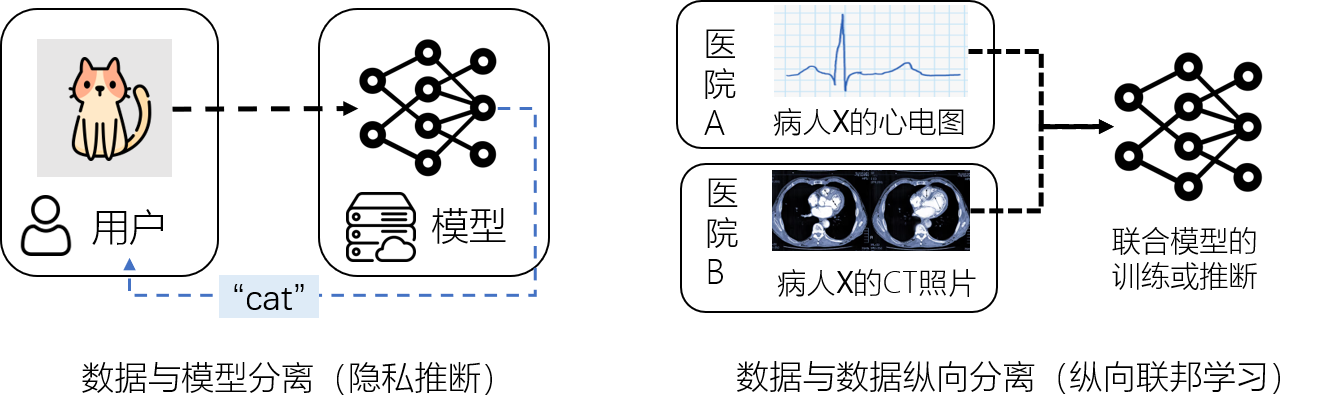
\includegraphics[width=1\linewidth]{Z_Resources/PPML-overview.png}
    \caption{本文主要研究的隐私保护场景}
    \label{fig:intro:ppml-overview}
\end{figure}


根据模型和数据的切分方式,人工智能应用中的隐私保护主要可以分为三个场景,分别是数据与模型分离的“隐私推断(Private Inference)”场景~\cite{mann_2023_secure_inference}、数据纵向切分(同一个样本的特征/标签列分布在不同参与方,模型参数也被切分给对应的参与方)的“纵向联邦学习(Vertical Federated Learning)”场景~\cite{liu2024vertical}、以及数据横向切分(拥有同样特征列的不同样本分布在不同参与方,模型参数全局共享)的“(横向)联邦学习(Federated Learning)”场景~\cite{yangqiang2019federated}。
%
%
其中数据与数据横向分离场景中的数据隐私问题已经有联邦学习这一较为成熟的解决方案~\cite{yangqiang2019federated}。
联邦学习的基础范式为联邦平均(Federated Averaging)算法~\cite{mcmahan_2017_fedavg},其通过多个参与方在本地训练模型然后在服务器上以参数平均等方式聚合,从而保护各个参与方的数据隐私。
%
虽然该方法实现简单,但是其应用场景局限在数据横向分布(各方拥有具有相同格式的不同样本)的模型训练阶段,且无法保护模型的隐私,因此具有一定的局限性。
%
而隐私保护机器学习(Privacy-Preserving Machine Learning)是解决人工智能应用中的隐私问题的更为通用的解决方案~\cite{al_2019_ppml,xu_2021_ppml},
其涵盖密码学~\cite{evans_2018_pragmatic_mpc}、联邦学习、拆分学习~\cite{vepakomma2018split}等多种技术,实现对人工智能模型训练或推断过程中的隐私保护,可以适配多种人工智能模型的训练和推断场景。
%
与联邦学习的场景互补,本文中所讨论的隐私保护机器学习方案往往考虑在单次计算中参与方较少的场景,对应数据与模型分离以及数据与数据纵向分离的场景,
如\autoref{fig:intro:ppml-overview}所示。
%
面向这些场景的隐私保护机器学习解决方案主要可以分为拆分学习、基于密码学的方法,以及密码学和非密码学的混合方法三类。
%
拆分学习将模型拆成多个部分,分别部署在不同的参与方上,各方通过交换中间结果进行模型的训练和推断。
%
因此拆分学习可以适用于数据纵向切分的情况,同样也可以适用于隐私推断的情况,因为各方只能获得部分的模型和隐层的数据,因此可以一定程度保护数据和模型的隐私。
%
密码学方法通过安全多方计算协议在输入数据(包含模型的输入和模型自身的参数)的情况下产生模型的计算结果,因此自然适用于各种隐私保护机器学习场景。
%
类似地,许多密码学和非密码学的混合方法也针对于数据纵向切分和隐私推断的情况。
%
因此,本文所研究的隐私保护机器学习方法均可以适用于数据纵向切分和隐私推断的情况,具备一定的通用性。


隐私保护机器学习的核心问题在于效率和安全。
%
基于密码学的隐私保护机器学习,能够达到很高的安全性,并且可以对安全性进行严格的数学证明,但是其需要复杂的多方交互计算以及昂贵的密码学加解密运算。
随着人工智能模型的规模日益庞大,许多类似ChatGPT的大规模模型被提出~\cite{chatgpt,touvron_2023_llama,duzhengxiao_2022_glm},其对计算能力的要求逐步提升,导致基于密码学方法的效率往往难以达到实用的标准~\cite{hou2023ciphergpt}。
%
而拆分学习以及其他混合方法相比密码学方法有着较高的效率,但是其安全性缺少严格的证明,许多研究也提出了针对这些方法的攻击方法~\cite{hezecheng_2019_model_inversion_attack,abuadbba2020can_split,wong_2020_lwe_model}。
同时,当前对于拆分学习效率优化的研究也较为缺少。
%
上述的效率和安全问题制约了隐私保护机器学习的应用,因此如何更好地平衡隐私保护机器学习的效率和安全,是当前人工智能隐私领域亟待解决的问题。
%
通过优化隐私保护机器学习的效率和安全,可以使得人工智能的应用更加广泛,并且更好地保护用户的隐私权和人工智能公司的数据及模型资产,推动人工智能产业可持续发展。


